% !TEX root = template.tex

\section{Function}

First, we fetched GO annotations~\cite{gene_ontology} for both our family proteins and the entirety of the SwissProt database~\cite{swissprot}. To have a more complete representation, we then expanded these GO annotations by parsing the ontology tree~\cite{obo_parser} and adding the ancestor GO terms of each initially found GO term. In order to calculate the enrichment of each GO term in our family compared to the ones found in the SwissProt database, we used Fisher's exact test~\cite{fisher_test}. The contingency table was setup with rows defining the existence of a GO term and columns whether the protein is in the family or not (Table~\ref{tab:contingency}). 
\begin{table}[H]
    \centering
    \small
    \begin{tabular}{lccc}
        \toprule
         & Protein in family & \multicolumn{2}{c}{Protein not in family} \\
        \\
        \midrule
        Has GO term & $a$ & \multicolumn{2}{c}{$b$} \\
        No GO term & $c$ & \multicolumn{2}{c}{$d$} \\
        \bottomrule
    \end{tabular}
    \caption{Contingency table}
    \label{tab:contingency}
\end{table}
The null hypothesis was, for each GO term independently, that the proportion of proteins with this GO term in our family is the same as the proportion of proteins in the SwissProt dataset with this GO term. The alternative hypothesis was defined using right-tail, i.e., our family has a higher proportion of this GO term than SwissProt, and two-tail, i.e., the proportion is different (either higher or lower). The enrichment value was then calculated as:
$$
\dfrac{family\_proportion}{swissprot\_proportion}
$$
which was ultimately used as the weighting values for the word cloud showing only terms with p-values lower than $0.05$ for both two-tail and right-tail, which we refer to as enriched terms (Fig.~\ref{fig:go-wordcloud}). Furthermore, we reported the most enriched branches of the ontology tree based on the enriched terms (Fig.~...). For each GO term, we parsed the ontology tree~\cite{obo_parser} up to the root and added the GO term itself as an enriched child to each found ancestor. After this process, we selected only branches that had more than $2$ enriched children and a maximum depth of $3$ to filter for high-level terms. A selection of $10$ of these branches, scored by the sum of the negative logarithm of the two-tail p-values of their children, can be seen in Table~\ref{tab:go_terms}.

\begin{table}[h!]
    \centering
    \resizebox{1\linewidth}{!}{%
    \begin{tabular}{|l|c|c|c|}
        \hline
        \textbf{GO Term} & \textbf{Depth} & \textbf{Enriched} & \textbf{Score} \\
        \hline
        biological\_process & 0 & 212 & 2654.64 \\
        cellular process & 1 & 83 & 1685.44 \\
        molecular\_function & 0 & 42 & 1407.35 \\
        metabolic process & 2 & 58 & 1161.52 \\
        catalytic activity & 1 & 20 & 1066.89 \\
        hydrolase activity & 2 & 17 & 1006.90 \\
        primary metabolic process & 3 & 40 & 993.51 \\
        hydrolase activity, ester bonds & 3 & 15 & 916.11 \\
        biological regulation & 1 & 68 & 529.29 \\
        regulation of biological process & 2 & 64 & 515.90 \\
        \hline
    \end{tabular}%
    }
    \caption{Top 10 enriched branches}
    \label{tab:go_terms}
\end{table}



\begin{figure*}[h!]
    \centering
    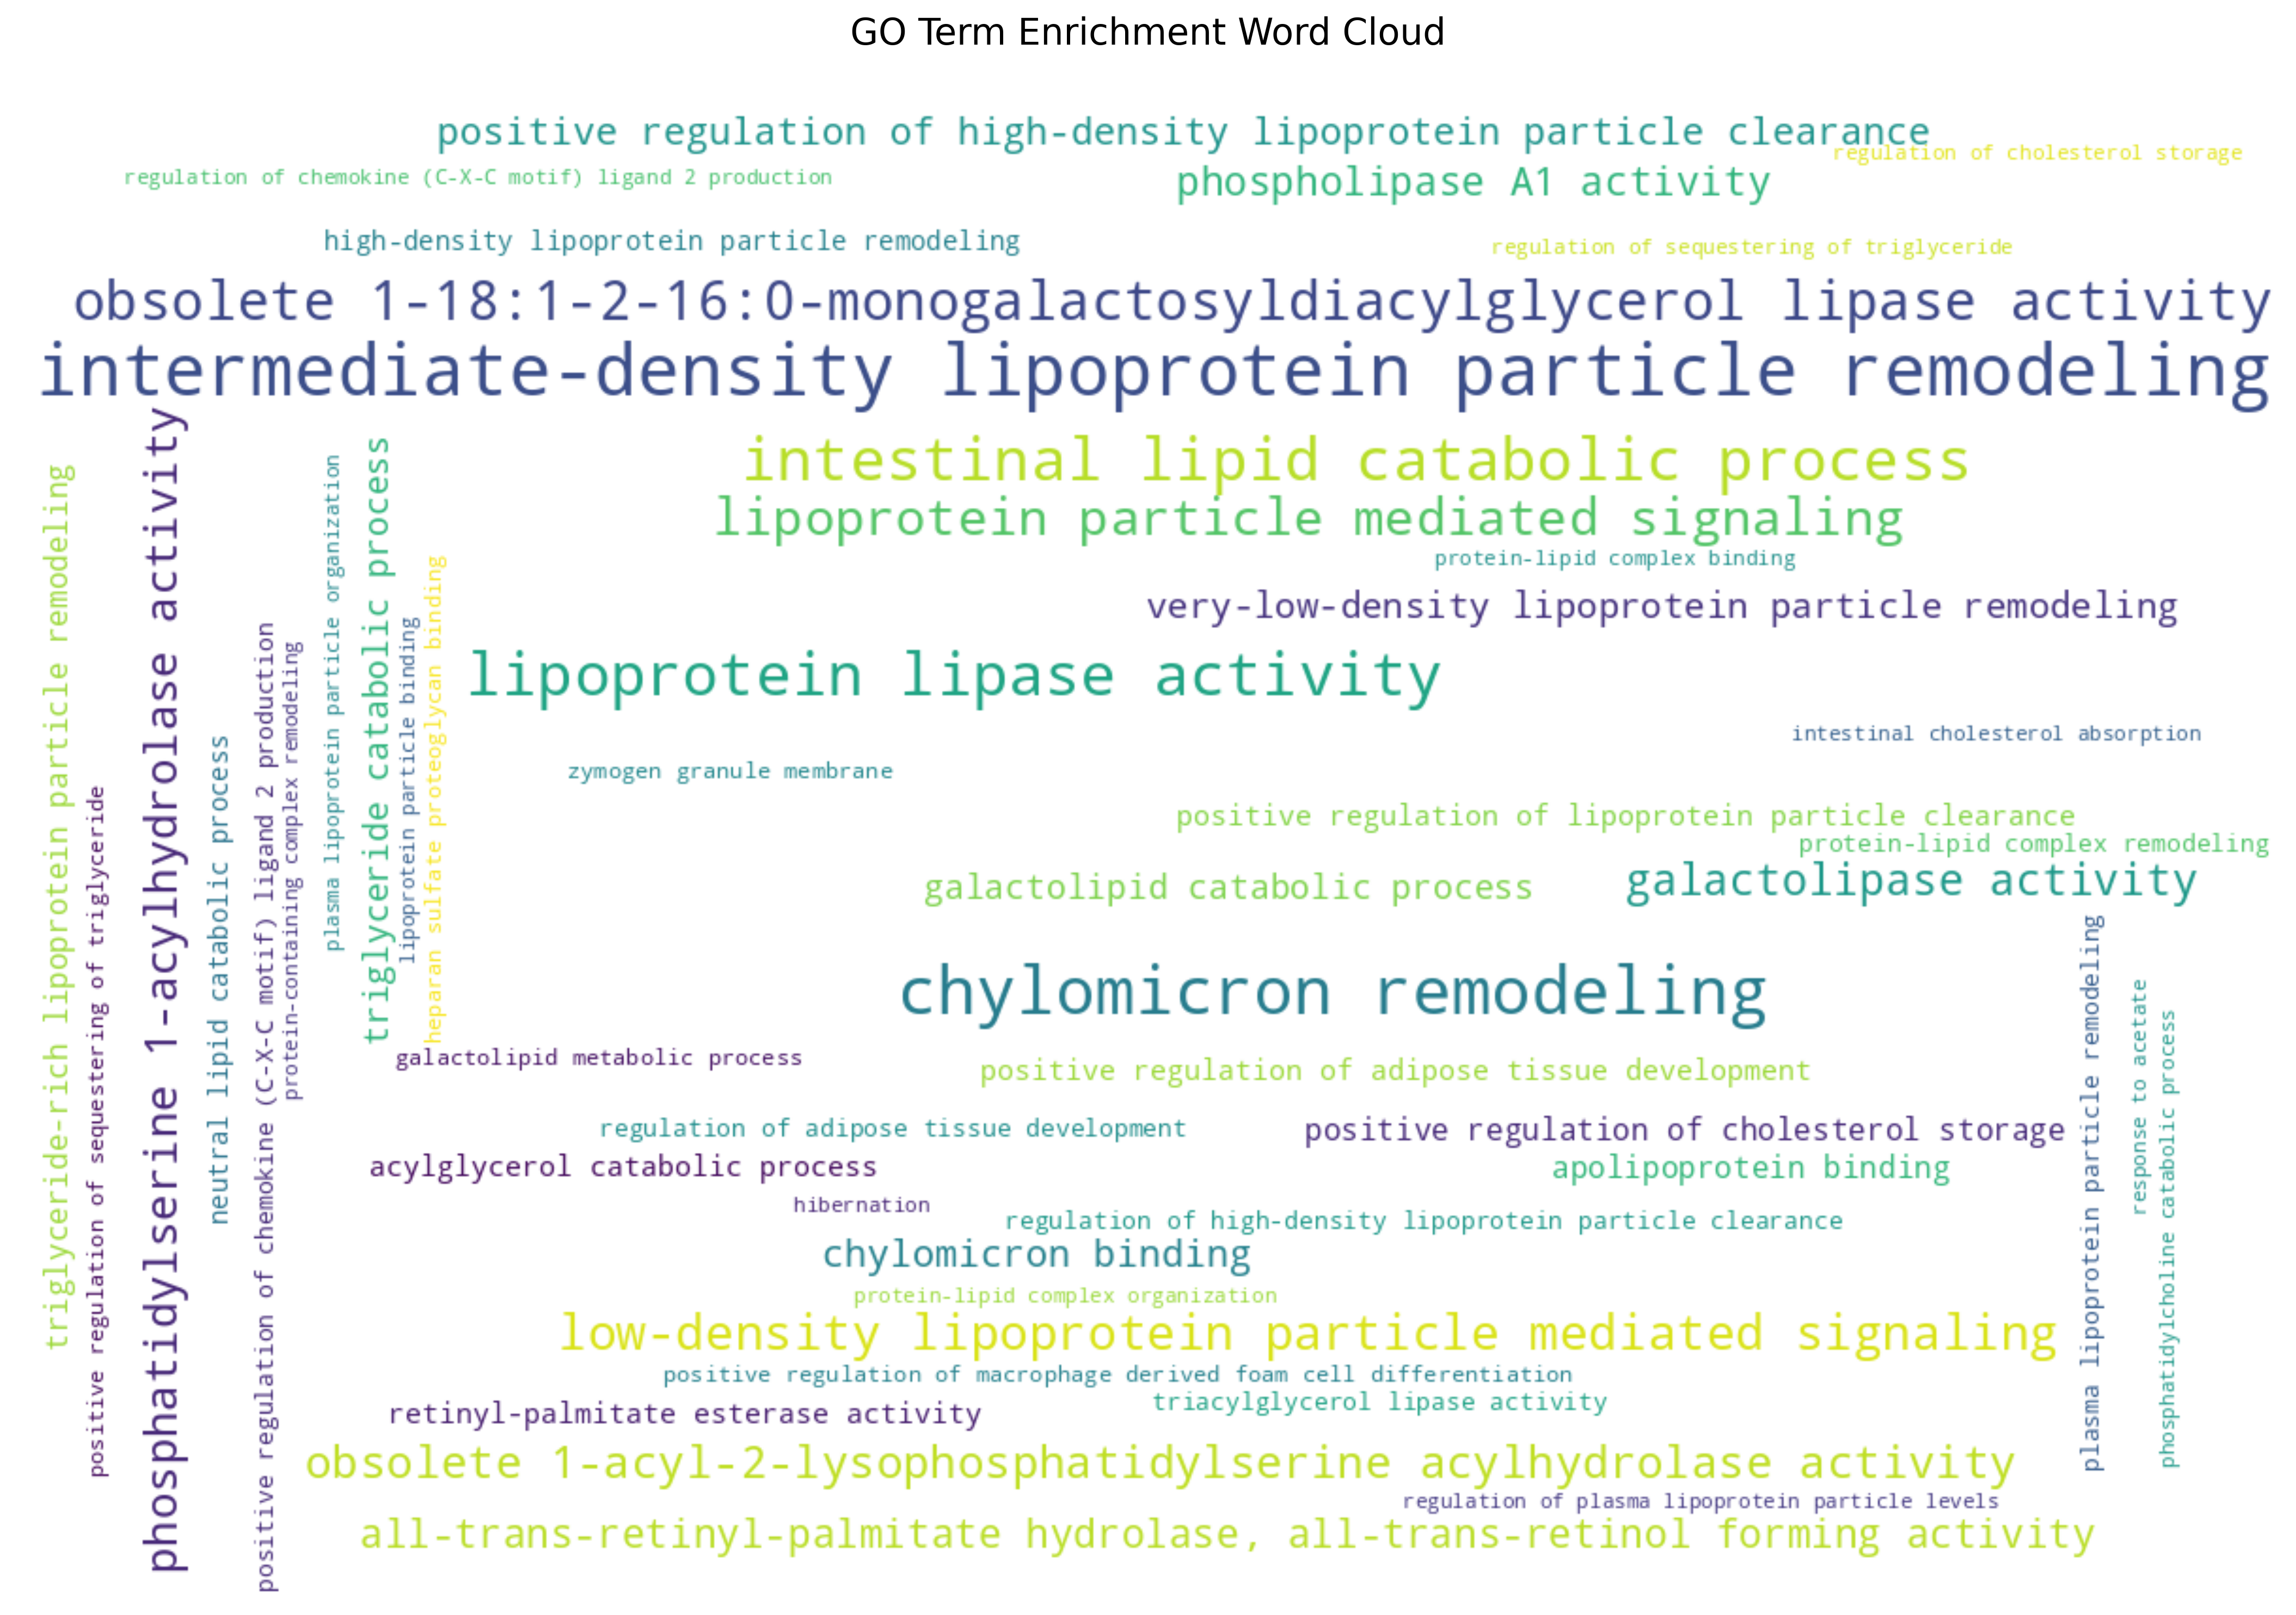
\includegraphics[width=0.8\textwidth]{images/go_enrichment_wordcloud.png}
    \caption{Word cloud visualization of enriched GO terms. The size of each term represents its relative frequency or significance, with larger text indicating higher enrichment. Terms are related to lipoprotein metabolism, lipase activity, and various cellular processes.}
    \label{fig:go-wordcloud}
\end{figure*}
